\documentclass[]{article}
\usepackage{fullpage}
\usepackage[authoryear]{natbib}
\usepackage{setspace}
    \doublespacing
\usepackage{hyperref}
\hypersetup{
    colorlinks,
    citecolor=black,
    filecolor=black,
    linkcolor=cyan,
    urlcolor=cyan
}
\usepackage{amssymb,amsmath}
\usepackage{bm}
\usepackage{dcolumn}
\usepackage{booktabs}
\usepackage{url}
\usepackage{tikz}
\usepackage{todonotes}
\usepackage[utf8]{inputenc}
\usepackage{graphicx}
\usepackage{longtable}
\usepackage{todonotes}
\usepackage{lscape}
\usepackage{float}


\title{Getting it Right\ldots Eventually: Political budget cycles and financial crises in Europe}

\author{Christopher Gandrud \\ \emph{City University London} \\ \emph{Hertie School of Governance}\footnote{Please contact Christopher Gandrud
(\href{mailto:christopher.gandrud@city.ac.uk}{\nolinkurl{christopher.gandrud@city.ac.uk}}).}
\and
Mark Hallerberg \\ \emph{Hertie School of Governance}}

\begin{document}

\maketitle

\begin{center}
    \textbf{Very Early Working Draft \\ for Texas A \& M University: Fiscal Policy in Europe Workshop}
\end{center}

\begin{abstract}
    Elected governments have incentives to classify loss-making endeavors, such as public industries and pension schemes, as off of the public balance sheet. Doing so improves the appearance of the government to cost-conscious voters as fiscally restrained. This is especially true during financial crises given their typical expense and the type of policy options available to assist troubled financial institutions, such as bad banks, nationalization. We examine revisions that to government debt and deficit figures made by the European statistical agency--Eurostat. These revisions frequently occur because this politically independent agency re-classifies organizations as within the government sector, when a national government had originally classified it as off.  We find that debt figures are more likely to be revised upward for years close to national elections. This effect is strengthened further by financial market stress.
\end{abstract}

\section{Introduction}

\section{Political budget cycles and fiscal gimmicks}

\cite{DeCastro2013} \cite{Alt2014}

\section{Cost-shifting during financial crises}

\cite{GandrudHallerberg2016}

\section{Hypotheses}

\begin{quote}
    $H_{1}$: Debt revisions will be greater for years closer to national government elections.
\end{quote}

\begin{quote}
    $H_{2}$: Debt revisions will be even greater for years closer to elections when there is high financial market stress.
\end{quote}

\section{Empirical tests}

To test these hypotheses we gathered all of the revisions that Eurostat made to EU member debt and deficit figures from 2003 through 2013. [WEBSITE URL] Eurostat publishes revisions bi-annually--typically once at the end of April and again again in late October. These revisions cover government finance statistics released within the previous four years.

\begin{figure}
    \caption{Marginal Effect of Election Timing (years to election) at Various Levels of Financial Market Stress on Debt Revisions}
    \label{me_finstress_elect}

    \begin{center}
        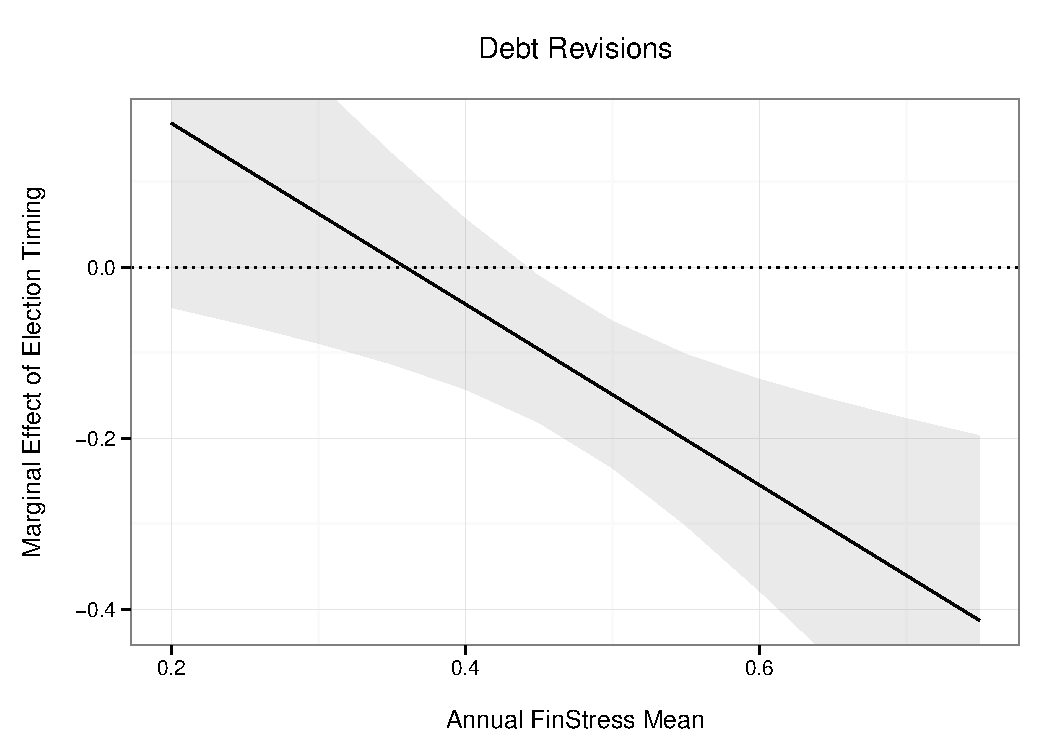
\includegraphics[scale=0.6]{figures/finstress_elect_me.pdf}
    \end{center}

{\scriptsize{Shadded area represents 95\% confidence interval.}}

\end{figure}


\section{Conclusion}


\clearpage

\bibliographystyle{apsr}
\bibliography{main.bib}

\end{document}
